\documentclass[12pt]{article}
\usepackage[margin=1in]{geometry}
\usepackage{amsmath, amssymb, amsthm, tcolorbox, lastpage}
\usepackage{fancyhdr, accents}
\usepackage{natbib, hyperref}
\usepackage{graphicx}
\usepackage{minted}


\pagestyle{fancy}
\setlength{\headheight}{40pt}

\newcommand{\ubar}[1]{\underaccent{\bar}{#1}}

\newcommand\tab[1][1cm]{\hspace*{#1}}

\title{CSC111H1-S Winter 2021 - Fundamentals of Computer Science 2 \\ Course Project Report}
\author{
  Ching Chang\\
  \and
  Letian Cheng\\
  \and
  Arkaprava Choudhury\\
  \and
  Hanrui Fan
}
\date{\today}

\begin{document}

\maketitle

\newpage

\lhead{Ching Chang, Letian Cheng \\ Arkaprava Choudhury, Hanrui Fan}
\rhead{CSC111H1-S Winter 2021 \\ Fundamentals of Computer Science 2 \\ Course Project Report}
\cfoot{\thepage\ of \pageref{LastPage}}

\begin{enumerate}
\item \section*{Part 1}
\textbf{Animmend - An interactive anime recommendation system.}

Ching Chang, Letian Cheng, Arkaprava Choudhury, Hanrui Fan

\newpage

\item \section*{Part 2: Problem Description and Research Question}
\begin{enumerate}
    \item \textbf{Overview of Background}
    
    \quad Anime is a genre of film and television animation that originated in Japan. Its wide range of storyline and unique art style has attracted over 20 millions audiences since 2018 \citep{Ani18}, and has been significantly scaling in multiple directions in the past 17 years \citep{Ell18}. With over 210 anime published last year in 2020 \citep{wiki21}, there are currently over 17,548 anime in the world \citep{MyA21} — way too many for anyone to pick!
    
    \item \textbf{Problem and Motivation}
    
    \quad This is a problem for both the audience and the producers of the anime who put in their blood and sweat into creating the work, only for it to be buried down in the monstrous pile of anime that are endlessly being published. Although there are anime-recommendation websites and applications out there that recommend users anime they might like based on their watch history, they tend to favour the trend and popular choices. This causes the established studios to self-perpetuate on the top of the pyramid scheme, while the rest that fails to make a good first impression end up at the bottom of the iceberg, forgotten. Much like every other film and television animation, anime is a form of fine arts medium where the authors, artists, and the production team splash their canvas with imagination and creativity. In a field with such freedom and originality, every anime has a meaningful story for someone in the world. Even the most terribly rated anime by the general could be a treasure to the right audience. However, it is difficult finding this so-called “right audience”. Anime with big names speak for themselves, so what the anime community lacks is a bridge between the unheard anime and the audience.
    
    \item \textbf{Our Goal}
    
    \quad To help mitigate this problem, we seek to create \textbf{an application that recommends unpopular anime based on the user’s input anime and relevant themes that they might be interested in.}
\end{enumerate}

\newpage

\item \section*{Part 3: Datasets}

\begin{itemize}
    \item Manami: An offline anime database \citep{manami}
    
    \textbf{Format:} This dataset's format is json. \href{https://gist.github.com/RealFakeAccount/cf34244d17039e78512428a1cf51d95f}{Data Example saved on GitHub}
    
    \textbf{Description:} 
    This source is used for retrieving each anime's title, thumbnail url, tags, and url to a webpage containing information about the anime. The rest of the data is ignored
    
    \item full.json: The parsed version of the Manami dataset, generated by our parse.py program
    
    \textbf{Format:} This dataset's format is json. 
    
    \textbf{Description:} This dataset is the output of parse.py. parse.py extracts the the title, url, thumbnail url, and tags of each anime from the original database and writes to a new json file. Note that anime with 0 tags will be removed
    
    \emph{A small sample of this dataset is called small.json}
    
    \item full\_graph.json: the serialize data of graph object
    
    \textbf{Format:} This dataset's format is json.
    
    \textbf{Description:} This dataset is the output of \emph{Graph.serialize} in Graph.py, and is used by the function \textit{load\_from\_serialized\_data} later. Since it takes roughly 17 seconds to calculate the similarity scores between all anime on 24 core cpu, we decided to calculate the similarity once, and save the results into a file that we can read from in the future.
    
    This file stores the attribute of the graph, \_anime: dict[str, Anime], which contains all attributes in the Anime class:
    
    \begin{minted}
        [
        frame=lines,
        framesep=2mm,
        baselinestretch=1.2,
        fontsize=\footnotesize,
        ]
        {python}
        
        title: str  # name of anime
        url: str  # url of anime on MAL
        thumbnail: str  # thumbnail
        detail: str  # introduction to the anime
        neighbours: list[str]
    \end{minted}

    \emph{We have a small sample of this dataset in small\_graph.json}
    
\end{itemize}
\newpage

\item \section*{Part 4: Computational Overview}

\begin{text}

\begin{itemize}
    \item parse.py
    \begin{itemize}
        \item parse\_json
        
            The \emph{parse\_json} function is used for processing the original Manami dataset. \textbf{New library, json, is used here} to read from and write to a json file. It opens the original Manami dataset, creates an empty dictionary, and add every part of the data we need (title, url, thumbnail, tags, and description) into the dictionary, while ignoring all the parts we do not need. After reading through the whole original json, we write the mutated dictionary into a new file.
            
        \item generate\_dataset
        
            The \emph{generate\_dataset} function is used for generate serialized dataset for the graph drawing. It calls graph.py and do a computation from scratch, then serialize them into file.
            
        \item update\_graph
        
            The \emph{update\_graph} function is used for update graph based on previous user feedback.
    \end{itemize}

    
    \item Anime class in anime.py
    
    We used a graph structure to represent the collection of anime in our database. 
    
    Each vertex in the graph represents a single anime. We create a custom class “\texttt{Anime}” with public instance attributes including the anime's title (\texttt{str}), its review score on Manami (float), and a list of similar anime. We also include a private instance attribute, which is a dictionary mapping each relevant tag for the anime to a certain weighting. The dictionary is always normalized, i.e. the sum of the squares of the weightings is constant, which is implemented with the help of the helper function \texttt{normalize\_dict}. 
    
    We defined the ``similarity" of one anime with other anime as the sum of the products of the weightings corresponding to tags that both anime have in common. For instance, suppose that \texttt{a1} and \texttt{a2} have tags $t_1, \ldots, t_k$ in common with corresponding weights $w_{1,1}, \ldots, w_{1,k}$ in \texttt{a1} and $w_{2,1}, \ldots, w_{2,k}$ in \texttt{a2}. Then, we define:
    \begin{align*}
        similarity(a_1, a_2) &= \prod_{i=1}^k w_{1, i} \cdot w_{2, i}
    \end{align*}
    
    This approach is partly inspired by the vector space model used in search engines \citep{vspace}. The method \texttt{calculate\_similarity} in the anime class is a translation of this mathematical definition into Python code.
    
    As explained later in further detail, users can provide feedback on the recommendations, and the program automatically re-adjusts the weighting of each tag using vector normalization, and recomputes the similarity with other anime. This is done by the methods in the \texttt{Anime} class \texttt{adjust\_positive\_feedback} and \texttt{adjust\_negative\_feedback}. A positive feedback would increase the weightings of all relevant tags and a negative feedback decreases the weightings of all relevant tags.
    
    An anime's neighbours (i.e. the \texttt{neighbours} attribute) consists of the animes with the highest similarity with this anime.
    
    \item graph.py, Graph class and initialize graph

    There are several important functions in The \texttt{Graph} class.
    
    \begin{itemize}
        \item Graph.get\_anime\_description
        
            This function requires us to retrieve anime descriptions in real time, by making http requests. For that, \textbf{we use two new libraries: \textit{requests} and \textit{BeautifulSoup} here}. We first manually inspected the html structure of the websites that we are making the http requests to, and pre-defined the sections of the websites to parse from, for 4 different websites. As users click on the anime in our visualization, we will make http requests using the \textit{requests} library. With the returned data from the http requests, we then use \textit{BeautifulSoup} to parse and retrieve the description of the anime.
            
        \item Graph.serialize
        
            This function uses \textit{json} again in the same manner as we used it in \textit{parse.py}. We create an empty dictionary and iterate through each Anime in the graph, filling the dictionary with all the data contained in each anime, and write the dictionary into a json file. This is to save the loading time of running this program in the future, since calculating the similarity score between anime can take a very long time. By saving the graph data into a file (serializing), we can load directly from this data the next time we run the program, to avoid doing all the calculations again on initialization. Along with this method, we also implemented \textit{load\_from\_serialized\_data}, which uses \textit{json} to read from the serialized data, and construct the graph using it. Since the serialized data is obtained from the previous graph state, which is guaranteed to be a valid graph, we figured that it would be more efficient to modify \textit{Graph.add\_neighbour} from the implementation that we learned from class. From class, the method for inserting an edge between two vertices was to check that both vertices existed, then add each vertex to another one's set of neighbours. However, in our case, since we already know that the two vertices must exist (since the data is from the previous graph state), and we need to insert the neighbours in a specific order (descending similarity score), we modified the implementation such that \textit{Graph.add\_neighbour} is only one-directional. It only adds the anime associated to second parameter to the first parameter's list of neighbours, without adding the anime associated to the first parameter to the second parameter's list of neighbour. Calling this method on its own would seem error-prone, however, since we are using this method to load the serialized graph, it is error-free and more efficient.
            
        \item Graph.sort\_neighbours\_multiprocess
        
            This function uses \textit{multiprocessing} to speed up the calculation. This function needs to call Graph.\_sort\_neighbours, which has a time complexity of O(nlogn), n times. We have n equals to 31016. This should not be a big problem for languages like go and cpp. However, it takes more than 30 minutes for python. To solve this problem, we rewrite this function using multiprocessing.Pool. We open a process pool with cpu.count() - 1 numbers of process (-1 is for stability). After using multiprocessing.Pool.map to auto assign each anime with process, We assgn the result into the self.\_anime
            
        \item Graph.\_sort\_neighbours
        
            This function uses sort to sort out the most NEIGHBOUR\_LIMIT related animes for each anime.
            
        \item Graph.store\_feedback
        
        \item adjust\_weighting
        
        \item Graph.draw\_graph
    \end{itemize}
    

    \item visualization.py and interactive
    
    ...
\end{itemize}

\end{text}

\newpage

\item \section*{Part 5: Instructions for obtaining datasets and running the program}

\begin{text}
Please install all libraries under requirements.txt. Then,

Download the zip file using following credentials:

Claim ID: CF88gEU9dbhgAMnJ

Claim Passcode: NotYkSiXVc2BZ7Pb

or download from following link: https://uoftctf.org/data.zip

After unzip this file, you should have a folder contains the following files:

\begin{itemize}
    \item full\_graph.json
    \item full.json
    \item original.json
    \item small\_graph.json
    \item small.json
\end{itemize}

Finally, for the main.py, you have several options: 

If you want to test the parse.py and generate data from scratch, uncomment the line that contains generate\_dataset

If you have made some feedback and want to regenerate graph, uncomment the line contains update\_graph

Then, test server for dash app would run. It will automatically open a port. You should see a website.

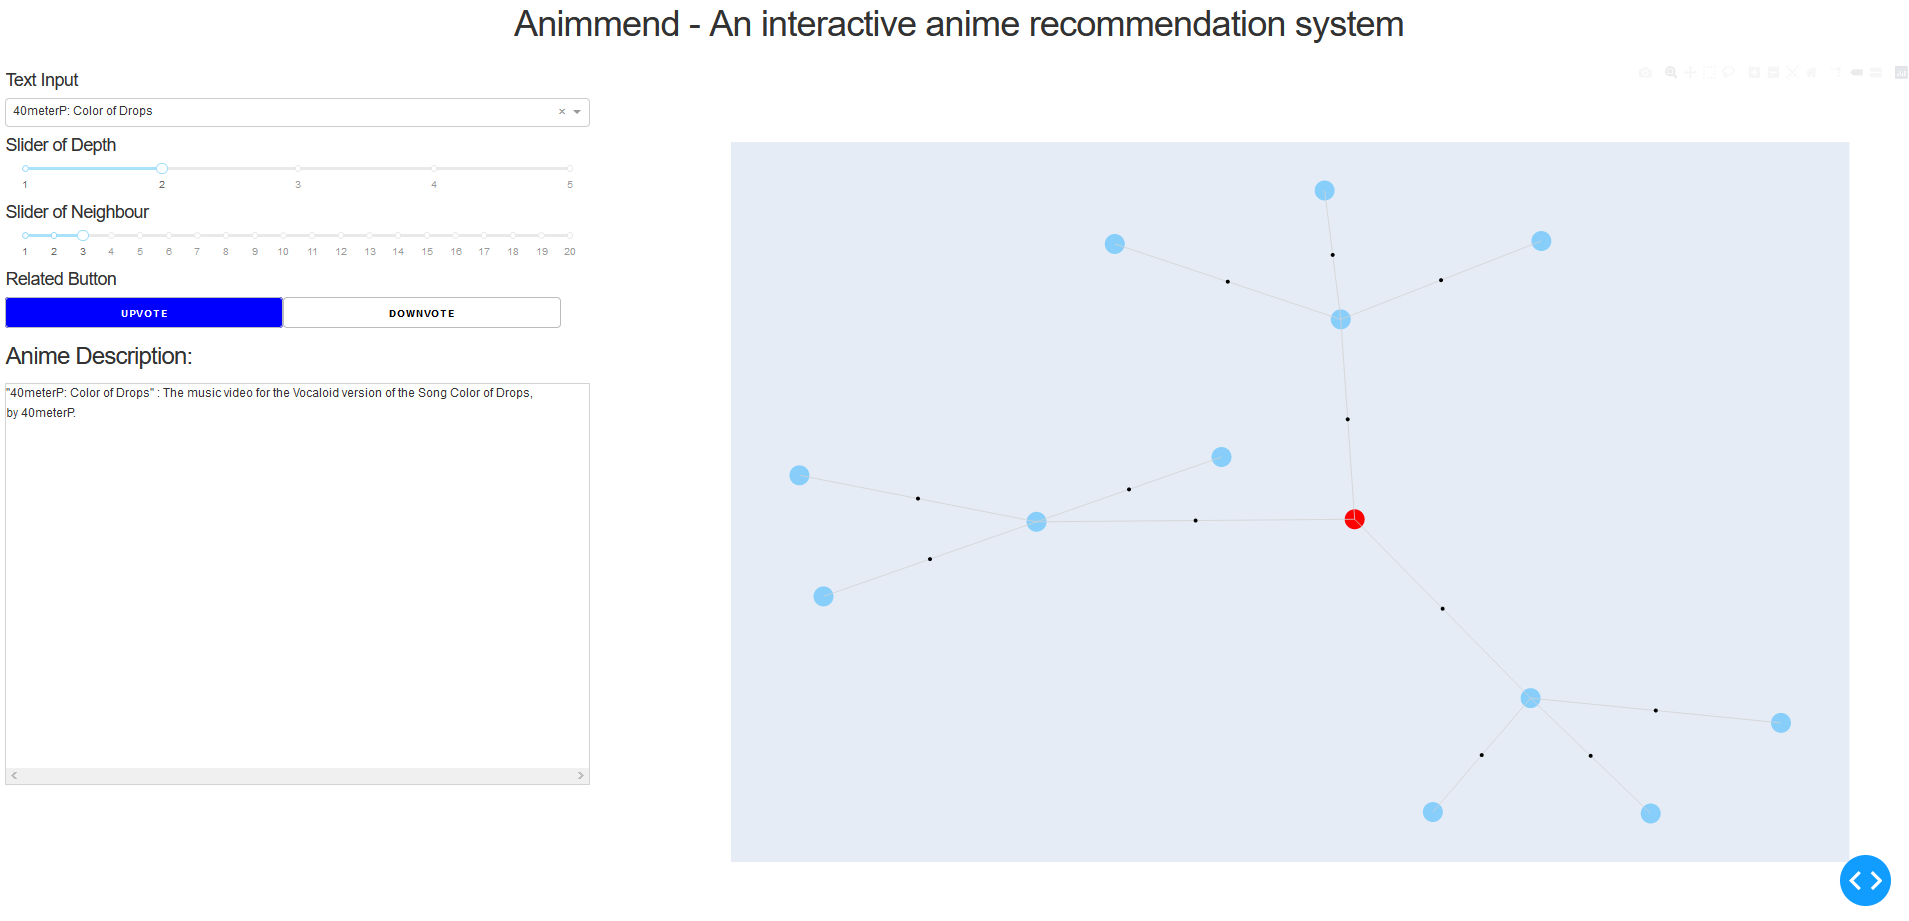
\includegraphics[scale=0.3]{sample}

On the left side, you got:

\begin{itemize}
    \item Text input: 

    you can select animes it have or type your favorite anime.

    \item Slider of depth: 

    you can change the depth of the graph (it's a tree actually) to get more recommendations.

    \item Slider of neighbour:

    you can change the number of edges for each node.

    \item feedback:

    after hovered into one anime, you can give feedback to the recommendation- either upvote or downvote. The feedback will update the graph later.

    \item Anime description:

    Hover into one anime, and the program will fetch description online. Note that the response time depends on your network connection.
\end{itemize}

On the right side, you got the graph. The red node is the current shell of the graph. The small black nodes store the similarity value of edge. The blue nodes are the recommendations.

You can click blue nodes to update the shell of graph.

\end{text}

\newpage

\item \section*{Part 6: Changes from Phase 1}

\begin{text}

\begin{enumerate}
    \item Edges...
    \item 
\end{enumerate}

\end{text}

\newpage

\item \section*{Part 7: Discussion}

\begin{text}

% discuss, analyse, and interpret the results of your program
%Do the results of your computational exploration help answer research question?
%What limitations did you encounter, with the datasets you found, the algorithms/libraries you used, or other obstacles?
%What are some next steps for further exploration?

\emph{\textbf{Do the results of your computational exploration help answer this question?}}

...

\emph{\textbf{What limitations did you encounter, with the datasets you found, the algorithms and libraries you used, or other obstacles?}}

...

\emph{\textbf{What are some next steps for further exploration?}}

\begin{enumerate}
    \item efficiency...
    \item implementation of symmetric version of similarity...
    \item updating anime graph with new anime...
\end{enumerate}

\end{text}


\maketitle

\newpage

\bibliography{references}
\bibliographystyle{apalike}

\end{enumerate}

\end{document}